\documentclass[a4paper,12pt]{article}

\linespread{1.5}
\emergencystretch=1cm

\usepackage[T2A]{fontenc}
\usepackage[utf8]{inputenc}
\usepackage[english, ngerman, russian]{babel}

\usepackage{amsfonts}
\def\R{\mathbb{R}}
\def\C{\mathbb{C}}

\usepackage{amsmath} % dfrac

\usepackage{graphicx}
\graphicspath{ {./assets/} }

\usepackage{biblatex}
\addbibresource{references.bib}

\usepackage{csquotes}

\usepackage{amsthm}
\newtheorem*{theorem}{Теорема}
\theoremstyle{remark}
\newtheorem*{remark}{Замечание}

\usepackage[left=3cm,
            right=1cm,
            top=2cm,
            bottom=2cm]{geometry}

\begin{document}

\begin{center}
  {\small МИНИСТЕРСТВО ОБРАЗОВАНИЯ И НАУКИ РОССИЙСКОЙ ФЕДЕРАЦИИ}

  \text{Федеральное агентство по образованию}
  \vspace{0.1cm}

  {\small МОСКОВСКИЙ ГОСУДАРСТВЕННЫЙ УНИВЕРСИТЕТ ИМ. М. В. ЛОМОНОСОВА}
  \vspace{4.5cm}


  {\Huge\textsc{РЕФЕРАТ}\\[5mm]}

  {\Large  Основы общей теории функций одной комплексной
    переменной. Бернхард Риман.}
  \bigskip

  \vspace{0.25cm}
\end{center}

\vfill

\hfill\begin{minipage}{0.55\linewidth}
  Работу выполнил: \\
  студент механико-математического \\
  факультета 5 курса\\
  Шерстобитов Андрей Сергеевич\\
  Преподаватель:\\
  кандидат физико-математических наук \\
  Смирнова Галина Сергеевна\\
\end{minipage}

\vfill

\begin{center}
  Москва, 2024 г.
\end{center}

\thispagestyle{empty}
\newpage

\tableofcontents

\thispagestyle{empty}
\newpage

\section{Введение}

\subsection{Предисловие}

Впервые я услышал имя Бернхард Риман, когда я изучал основы
математического анализа на первом курсе механико-математического
факультета. Неожиданным для меня было услышать упоминание
``Гипотезы Римана'' в контексте теории чисел,
и тогда это имя заинтриговало меня. Кто был этот Риман,
и почему его идеи оказались такими значимыми для математики?

Оказалось, что Бернхард Риман был не только новатором в математическом
анализе, но и человеком, который сделал значительный вклад в множество
других областей математики, включая дифференциальную геометрию и комплексный анализ.
Именно его работа <<Основы общей теории функций одной комплексной
переменной>> \cite{Dissertation} стала основой
для понимания многих концепций в современной теории функций.

Когда я начал изучать эту тему глубже, я понял, что комплексный анализ
имеет широкое применение в различных областях науки и техники:
от физики и инженерии до финансов и компьютерных наук. Работа
Римана содержит в себе ключевые идеи, которые впоследствии легли
в основу теории аналитических функций, топологии и даже квантовой
теории поля.
\begin{quotation}
  О Римане еще в большей степени, чем о Гауссе\footnote{
    Карл Фридрих Гаусс (нем. Johann Carl Friedrich Gauß), 1777—1855 --
    немецкий математик, механик, физик, астроном и геодезист, прозванный ``Принцем математики''
    за его глубокий вклад в разные области математики.
  }, можно сказать,
  что он стоит на грани двух эпох в математике, сочетая в себе их
  противоречия: он держит плотную связь с классиками, ..., но еще
  более тесные узлы связывают его с последующими поколениями
\end{quotation}
-- так говорит о нем В. Л. Гончаров\footnote{
  Гончаров Василий Леонидович, 1896—1955 --
  советский и российский учёный, педагог, математик, доктор физико-математических
  наук, член-корреспондент Академии педагогических наук РСФСР.
  Профессор Московского государственного университета.
} \cite{Essays}, переводчик выбранного мной для реферирования произведения.

Таким образом, изучение труда Римана помогает не только понять
развитие комплексного анализа, но и дает общее представление о том,
как математические идеи могут перекликаться между различными дисциплинами.
Мой реферат будет посвящен разбору этой работы Римана,
её значимости для современной математики и того,
как она повлияла на последующие исследования.

\subsection{Об авторе выбранного произведения}

Георг Фридрих Бернхард Риман (нем. Georg Friedrich Bernhard Riemann) родился
17 сентября 1826 года в городе Бреселенц, Нижняя Саксония,
Германия, в семье лютеранского пастора Фридриха Римана.
Риман был вторым из шести детей в семье, и с раннего возраста
проявлял необычайные способности к математике. В отличие от
своих сверстников, он мог решать сложные арифметические задачи
и демонстрировал глубокое понимание математических принципов.

\begin{figure}[h]
  \centering
  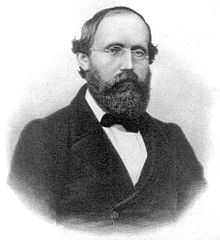
\includegraphics{Georg_Friedrich_Bernhard_Riemann.jpeg}
  \caption{Бернхард Риман (1863)}
\end{figure}

Первоначально Риман начал свое образование в сельской школе,
но вскоре перешел в гимназию в Ганновере, а затем в средней
школе в Люнебурге, там же изучал труды Эйлера\footnote{
  Леонард Эйлер (нем. Leonhard Euler), 1707—1783 --
  швейцарсий математик и физик. Считается одним из наиболее продуктивных математиков
  в истории, автором более 800 публикаций.
}, Лежандра\footnote{
  Адриен Мари Лежандр (фр. Adrien-Marie Legendre), 1752—1833 --
  французский математик. Его наиболее известные работы касаются законов квадратичной взаимности
  в теории чисел, а также функций Лежандра, которые используются
  в решении дифференциальных уравнений и применяются в физике.
} и других математиков.
Его учителя заметили его математический талант
и рекомендовали ему поступить в Гёттингенский университет,
где он начал свое высшее образование в 1846 году, сначала
изучая теологию, следуя по стопам своего отца.
Однако, вскоре он переключился на изучение математики,
вдохновленный лекциями Карла Фридриха Гаусса.
Позднее в 1847-1849 гг. уже в Берлинском университете слушал
лекции Дирихле\footnote{
  Иоганн Петер Густав Лежён Дирихле (нем. Johann Peter Gustav Lejeune Dirichlet), 1805—1859 --
  немецкий математик. Известен своими работами в области рядов Фурье, принципом Дирихле,
  а также исследованиями функционального анализа.
}, Штейнера\footnote{
  Якоб Штейнер (нем. Jakob Steiner) 1796—1863 --
  швейцарский математик, считается одним из основателей
  современной проективной геометрии. Известен своими работами по
  геометрическим построениям и теоремам о кривых и поверхностях.
}, Якоби\footnote{
  Карл Густав Якоб Якоби (нем. Carl Gustav Jacob Jacobi) --
  немецкий математик, внес вклад в область математического анализа, алгебры и теории эллиптических
  функций. Он был одним из первых математиков, кто продемонстрировал
  применение алгебры к анализу, а также развил теории матриц и определителей.
}. \cite{MathEncyclopedia}.

В 1851 году Риман защитил рассматриваемую нами диссертацию,
исследовал топологию поверхностей, и заложил основы современной
комплексной геометрии. Эта работа, отмеченная Гауссом, привела
к его сотрудничеству с выдающимися математиками, такими как
Дедекинд\footnote{
  Юлиус Вильгельм Рихард Дедекинд (нем. Julius Wilhelm Richard Dedekind) 1831—1916 --
  немецкий математик. Прославился благодаря введению понятия ``отрезков Дедекинда'',
  которые дали более строгий фундамент для определения вещественных чисел.
  Также развил теории колец и идеалов, которые в дальнейшем стали основой для алгебраической теории чисел.
} и Куммер\footnote{
  Эрнст Эдуард Куммер (нем. Ernst Eduard Kummer), 1810—1893 --
  немецкий математик. Ввёл понятия ``идеальных чисел'' и ``идеальных элементов'', понадобившиеся для разрешения проблем в теории чисел и алгебраической геометрии.
}. Дедекинд был его близким другом и сыграл важную роль в публикации
некоторых работ Римана после его смерти.

Риман продолжал работу в Геттингене, где в 1854 году он
прочитал свою знаменитую лекцию ``О гипотезах, лежащих в основании геометрии''.
В этой лекции он представил концепцию многомерных пространств -- многообразий,
разрабатывая основы римановой геометрии, которая впоследствии стала
фундаментом для теории относительности Эйнштейна\footnote{
  Альберт Эйнштейн (нем. Albert Einstein), 1879—1955 --
  немецкий физик-теоретик, известный за свою теорию относительности.
  Сделал значительный вклад в квантовую механику.
}. Риман продемонстрировал, как пространство может быть искривлено, что
оказало значительное влияние на развитие физики.

С 1859 года Риман был профессором в Геттингенском университете, читал
лекции по математической физике. Опубликовал свою знаковую статью <<О количестве
простых чисел, меньших данной величины>> \cite{Hypothesis}, в которой он предложил
гипотезу Римана, касающуюся распределения простых чисел. Эта гипотеза
до сих пор остается одной из самых известных нерешенных проблем
в математике, и множество исследователей потратили годы, пытаясь
найти её доказательство.

Риман был не только ученым, но и человеком с глубокими религиозными
убеждениями, унаследованными от своего отца.
Он вел скромный образ жизни и стремился к интеллектуальной скромности (из писем Дедекинда).

В 1866 году, во время путешествия в Италию, Риман скончался от туберкулеза
в возрасте 39 лет в городе Селаска. Несмотря на короткую жизнь, его наследие в математике
огромно. Его работы повлияли на такие области, как дифференциальная геометрия,
комплексный анализ, топология и теория чисел. Взаимодействие с выдающимися
математиками своего времени помогло ему развить идеи, которые продолжают
влиять на математику до сих пор.

\subsection{О выбранном произведении}

Работа Бернхарда Римана <<Основы общей теории функций одной комплексной переменной>> \cite{Dissertation}
является фундаментальной работой в области комплексного анализа.

Эта диссертация существенно повлияла на других математиков, таких
как Вейерштрасс\footnote{
  Карл Теодор Вильгельм Вейерштрасс (нем. Karl Theodor Wilhelm Weierstraß), 1815—1897 --
  немецкий математик, считается одним из основателей современной
  теории анализа, он внёс существенный вклад в определение предела, непрерывности, дифференцируемости и сходимости.
  Известен за работу по аналитическим функциям, особенно в области комплексного анализа.
} и Кляйн\footnote{
  Феликс Христиан Клейн (Кляйн) (нем. Felix Christian Klein), 1849—1925 --
  немецкий математик и педагог. Знаменит благодаря своей
  <<Эрлангенской программе>>, в которой предложил классификацию
  геометрий на основе теории групп.
}. Вейерштрасс, известный своими работами по теории функций,
разработал свой собственный строгий подход к комплексному анализу,
который иногда контрастировал с более геометрическим подходом Римана\cite{Contrasts}.
Кляйн, внесший вклад в развитие теории групп и геометрии, находился под
глубоким влиянием концепций Римана, особенно в отношении римановых
поверхностей и их приложений в топологии. Первое упоминание
бутылки Кляйна появилось в монографии <<О теории Римана
алгебраических функций и их интегралов>> \cite{Klein}.

Для данного реферата я буду использоваться книгой <<Б. Риман, Сочинения>> \cite{Essays} --
переводом с немецкого языка под редакцией, с предисловием, обзорной статьей
и примечаниями профессора Гончарова В.Л.

Так высказывается об этой книге А.П.Юшкевич\footnote{
  Адольф Павлович Юшкевич, 1906—1993 --
  советский и российский историк науки. Автор более 200 нучных работ
  по истории математики. Издатель трудов классиков математиков.
}:
\begin{quotation}
  При выборе материала В. Л. Гончаров включил в русское издание все основные
  мемуары, написанные самим Риманом, оставив в стороне лишь некоторые
  фрагментарные работы, а также обработки лекций Римана по дифференциальным
  уравнениям с частными производными, эллиптическим функциям и теории электричества и магнетизма. ...
  Статью свою В. Л. Гончаров посвятил общей характеристике научного
  творчества Римана. В ней имеется немало спорных моментов, но
  и много интересных замечаний и большой фактический материал.
\end{quotation}

\newpage
\section{Основы общей теории функций одной комплексной переменной}

Отличительной чертой работ Римана является иная концепция функции.
У классиков, таких как Эйлер, функция была неразрывно связана с формулой.
Функция существовала там, где формула имела смысл, и прекращала существовать,
когда формула переставала быть применимой. Эта концепция основывалась на непосредственной
связи между формулой и функцией, предполагая, что формула определяет функцию.
В этой парадигме функция была ограничена областью, где формула могла быть
применена.

Риман, под влиянием наставника Дирихле, принял новую концепцию функции.
В этом новом определении функция отделилась от аналитического представления.
Это означало, что одна и та же функция могла быть выражена различными формулами,
и одна и та же формула могла представлять разные функции в различных областях.
Важно, что Риман использовал идею однозначного соответствия между значениями
переменных. Он изменил подход к функциям, рассматривая формулу лишь как случайный
атрибут, а не как сущность функции. Таким образом, Риман стал описывать функции более
узкого класса, именно те, которые сейчас зовутся аналитическими.

Первый параграф Риман начинает с объяснения того, что функция
$w$ переменной $z$ определена тогда, когда для каждого значения
$z$ есть соответствующее единственное значение
$w$. Он добавляет к этому указание, что если $z\in A\subset\R$, а
$w$ меняется непрерывно, то и функция считается непрерывной в пределах интервала $A$.

Также он обращает внимание, что определение непрерывности в
интервале не подразумевает какого-либо фиксированного закона
между значениями функции. То, как функция продолжается за пределы
данного интервала, совершенно не определено.

Риман описывает условия, при которых комплексные функции могут
быть дифференцированы. Он показывает, как $\frac{dw}{dz}$
функции не зависит от конкретного значения дифференциала $dz$.
Он устанавливает это условие как основу своего определения комплексных
функций от комплексной переменной.

В следующем параграфе Риман представляет комплексные числа как точки плоскоти $\R^2$,
а отношение между функцией $w$ и переменной $z$, таким образом можно представить
как отображение соответствующих им плоскостей.

В третьем параграфе Риман дает геометрическую интерпретацию
свойства функции комплексного переменного. Он показывает с помощью
данного в прошлом параграфе представления то, что для
таких функций выполняются соотношения подобия между двумя
малыми частями плоскостей образа и прообраза отображения.

Далее Риман выводит критерий $\C$-дифференцируемости функции комплексного переменного.

\[\frac{\partial u}{\partial x} = \frac{\partial v}{\partial y}
  , \quad
  \frac{\partial v}{\partial x} = - \frac{\partial u}{\partial y} \]

Сейчас мы называем этот критерий условиями Коши\footnote{
  Огюстен Луи Коши (фр. Augustin Louis Cauchy), 1789—1857 --
  французский математик. Ввёл многие фундаментальные понятия
  и теоремы, такие как теорема Коши о контурных интегралах
  и критерий Коши сходимости.
}-Римана или условиями Даламбера\footnote{
  Жан Лерон Д’Аламбер (фр. Jean Le Rond D'Alembert), 1717—1783 --
  французский учёный, энциклопедист, философ, математик и механик.
  Прославился решением волнового уравнения и одноименненым принципом из механики.
}-Эйлера.
Из этих условий Риман вывод известные нам уравнения Лапласа\footnote{
  Пьер-Симон Лаплас (фр. Pierre-Simon de Laplace), 1749—1827 --
  французский математик и астроном. Его <<Трактат о небесной механике>> обобщил и расширил принципы Ньютона, применяя их
  к изучению движения планет и других астрономических объектов.
}
\[\frac{\partial^2 u}{\partial x^2} + \frac{\partial^2 u}{\partial y^2} = 0,\quad
  \frac{\partial^2 v}{\partial x^2} + \frac{\partial^2 v}{\partial y^2} = 0\]

В пятом параграфе Риман переходит к более сложным объектам:
вводится определение \textit{поверхности, разостланной
  на плоскости}, ныне известной нам как риманова поверхность.
Риман требует, чтобы листы такой поверхности не были соединенны по общей кривой,
то есть такая поверхность не может ни расщепляться, ни образовывать складки.

Помимо этого в параграфе Риман аккуратно вводит определения
\textit{совершенно определенных} прилегающих к кривой
листах поверхностей и \textit{точек ветвления}.
С помощью этих объектов Риман высказывает важное предположение:
\begin{quotation}
  Если задана граница поверхности так по своему положению, так и по направлению и если задано также положение точек ветвления,
  то тем самым поверхность или вполне определена,
  или же не исключено, что существует несколько поверхностей, облалающих указанной границей и указаиитыми точками ветвления;
  \textbf{число таких поверхностей во всяком случае конечно}.
\end{quotation}

\begin{figure}
  \centering
  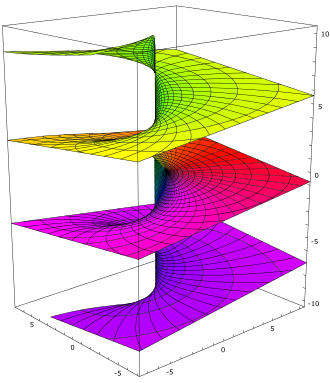
\includegraphics[width=0.25\textwidth]{Riemann_surface_log.png}
  \caption{Демонстрация точки ветвления на графике комплексного логарифма}
\end{figure}

В параграфе шесть Риман вводит формализм в топологии на таких поверхностях.
Математик рассказывает о связности поверхностей и её типах, дает определение разреза -- разбиения на несвязные участки.
Риман доказывает две теоремы, из следствия которых выводит значимый результат:
если число разрезов некоторой системы равно $n$, а число полученных после разрезывания
олносвязных частей поверхности равно $m$, то разность $n - m$, -- \textit{порядок связности}, -- остаётся
одной и той же, какова бы ни была система разрезов.

В седьмом параграфе Риман рассматривает функции на «поверхности $T$, разостланной по плоскости $A$».
То есть по сути каждой точке на поверхности он сопоставляет координаты $(x, y)$ её проекции на плоскость и рассматривает функции $X, Y$ на поверхности.
Эту теорему Риман формулирует следующим образом:

\begin{theorem}
  Пусть $X$ и $Y$ - две функции переменных $x, y$, непрерывные во всех точках разостланной по
  плоскости $A$ поверхности $T$, тогда справедлива следующая формула:
  \[ \int \left(\frac{\partial X}{\partial x} + \frac{\partial Y}{\partial y} \right)dT = -\int \left(X cos\xi + Ycos\eta\right)ds \]
  причём интеграл слева распространён на всю поверхность $T$, а интеграл справа берётся по
  всей границе, элемент которой обозначается через $ds$; что касается $\xi$ и $\eta$, то эти буквы
  обозначают углы, которые нормаль к граничной кривой, направленная внутрь поверхности
  $T$, делает с осями $x$ и $y$.
\end{theorem}

Здесь Риман требует, чтобы функции $X $ и $Y$ были гладкими,
но не требует гладкости частных производных этих функций,
в отличие от современной трактовки. Однако доказательство не
содержит противоречий в случае гладких функций $X$, $Y$ и гладкой границы

В последующих параграфах Риман делает ряд полезных свойств этого интеграла
при условии, если подынтегральная функция левой части обращается в ноль.
Эти условия будут соблюдаться для гармонических функций
на поверхностях, которые Риман рассматривает в 10 параграфе.
Действительно, пусть $u$ и $u'$ - гармонические функции почти во всех точках поверхности, тогда он рассматривает новые функции:

\[X = u\dfrac{\partial u'}{\partial x} - u'\dfrac{\partial u}{\partial x}, \quad Y = u\dfrac{\partial u'}{\partial y} - u'\dfrac{\partial u}{\partial y}\]

Но в таком случае выполнены следующие равенства:

\[\dfrac{\partial X}{\partial x} + \dfrac{\partial Y}{\partial y} = u\Delta u' -u' \Delta u = 0\]

Риман доказывает, что если функция $u$ имеет разрывы
в произвольных точках (не вдоль какой-либо кривой),
то этими разрывами можно пренебречь вследствие одного из выводов прошлого параграфа,
если произведение расстояния от точки некоторой точки $O$
до особенности и частных производных $u$ вдоль $x$ и $y$ стремится к нулю.

Далее Риман рассматривает функцию
\[\log{r_{(x_0, y_0)}(x,y)} = \log{((x-x_0)^2+(y-y_0)^2)}\]
где $(x_0, y_0)$ - некоторая произвольная точка. Эта функция гармонична во всех точках кроме $(x_0, y_0)$. На основании предыдущих рассуждений он выводит формулу:

\[u(x_0, y_0) = \frac{1}{2\pi} \int \left( \log{r_{(x_0, y_0)}}\frac{\partial u}{\partial p} - u \frac{\partial \log{r_{(x_0, y_0)}}}{\partial p}  \right)ds\]

где интегрирование ведётся по некоторому замкнутому контуру, внутри которого лежит точка
$(x_0, y_0)$, а оператор $\frac{\partial}{\partial p}$ - оператор дифференцирования по направлению нормали к границе,
направленной внутрь поверхности. Из этой формулы он получает знаменитую теорему о среднем значении гармонической функции, которая утверждает, что если  $\Delta u = 0$ в некоторой $U_\rho$
окрестности точки $(x_0, y_0)$, то $\forall\ 0 < r < \rho$ выполнена следующая формула:

\[u(x_0, y_0) = \dfrac{1}{2\pi} \int u(x_0 + r cos \phi, y_0 + r sin \phi) d\phi \]

На основании первой из двух последних формул Риман доказывает теорему:
\begin{theorem}
  Если функция $u$ на некоторой поверхности, разостланной без покрытий на плоскости $A$, удовлетворяет, вообще говоря, уровнению:
  \[\dfrac{\partial ^2 u}{\partial x ^2} + \dfrac{\partial ^2 u}{\partial y ^2} = 0\]
  или, точнее говоря, если
  \begin{enumerate}
    \item точки, в которых уравнение не выполняется, не заполняют никакой части плоскости,
    \item точки, в которых $u, \frac{\partial u}{\partial x}, \frac{\partial y}{\partial y}$, имеют разрывы, не заполняют никакой кривой,
    \item если имеются такие точки разрыва, то при бесконечно малых расстояниях $\rho$ точки $O$
          от точки разрыва величины $\rho \frac{\partial u}{\partial x}, \rho \frac{\partial u}{\partial y}$
          также бесконечно малы,
    \item не существует точек, в которых разрыв устранялся бы изменением одного значения,
  \end{enumerate}
  - то во всех точках, расположенных внутри данной поверхности, функция и конечна и
  непрерывна, так же как и её частные производные всех порядков.
\end{theorem}

На основе этой теоремы он доказывает единственность гармонической функции при заданных на некоторой кривой на поверхности значениях $u$ и $\frac{\partial u}{\partial p}$.

Изучив гармонические функции Римана возвращается к аналитическим функциям. Ранее он
показал, что если $u$ и $v$ - вещественная и мнимая части $\omega(z)$ соответственно, то $\Delta u = 0, \Delta v = 0$.
Теперь, используя результат, полученный для гармонических функций, он выводит следующий результат для аналитических функций:

\begin{theorem}
  Если функция $\omega$ переменной $z$ не имеет разрывов, образующих целые кривые,
  и, кроме того, для любой точки $O'$, где $z = z'$, нашей поверхности величина $\omega(z - z')$ при
  неограниченном приближении точки $O$ к $O'$ становится бесконечно малой, то функция
  вместе со всеми своими производными внутри поверхности конечна и непрерывна.
\end{theorem}

Нам эта теорема известна как теорема Римана об устранимой особой точке.

Далее профессор предлагает изменить последнее условие в теореме следующим образом:
пусть в некоторой точке $z = z'$ величина $\omega (z - z')$ уже не стремится к нулю при $z\rightarrow z'$.
Исходя из предыдущей теоремы, он показывает, что существует $n \in \mathbb{N}$ и набор комплексных чисел $a_1, ..., a_n$ таких,
что после вычитания выражения вида
\[\dfrac{a_1}{(z-z')^{\frac{1}{n}}}+ ...+ \dfrac{a_n}{(z-z')^{\frac{m}{n}}}\]
из $\omega(z)$ новая функция станет непрерывной в окрестности точки $z = z'$.
\begin{remark}
  Риман рассматривает только особенности типа полюс.
\end{remark}

Заметим, что все предыдущие результаты были получены Риманом только для областей на комплексной
плоскости. В следующем параграфе математик обобщает полученную им
теорию на любую поверхность $T$, разостланную по плоскости $A$.

Пусть задана аналитическая почти во всех точках функция
$\omega(z)$. Риман замечает, что если точка на поверхности не является точкой ветвления, то в её
окрестности функция удовлетворяет всем условиям доказанных ранее теорем.
Для точки ветвления он аккуратно строит отображение её окрестности на плоскость с помощью трюка из прошлого параграфа.
Таким образом, результат представляется в виде теоремы:
\begin{theorem}
  Если при бесконечном приближении точки $O$ к точке ветвления $(n-1)$ порядка
  $O'$ функция $w$ переменной $z$ становится бесконечной, то
  порядок бесконечности её в этой точке есть число, кратное $\dfrac{1}{n}$, и если,
  именно он равен -- $\dfrac{m}{n}$, то, прибавляя к $w$ выражение вида
  \[\dfrac{a_1}{(z-z')^{\frac{1}{n}}}+ ...+ \dfrac{a_n}{(z-z')^{\frac{m}{n}}}\]
  где $a_1, ..., a_n$ -- некоторые комплексные величины, мы получим
  функцию, непрерывную в точке $O'$.
\end{theorem}

В пятнадцатом параграфе своей работы он показывает новый подход к описанию функций на римановых поверхностях. Пусть на поверхности $T$ задана аналитическая функция $\omega = u + iv$.
Зафиксируем точку $P \in T$. Этой точке соответствует точка $Q$ на плоскости с координатами
$(u, v)$. Можем считать, что точка $Q$ расположена не на самой плоскости, а на некоторой поверхности $S$, разостланной по этой плоскости. Теперь соединим точку $P$ с некоторой другой точкой
$P' \in T$ тогда на поверхности $S$ возникает кривая, конец которой мы обозначим $Q'$. Сопоставим точке $P'$ точку $Q'$. Таким образом, отображение $\omega$ порождает отображение римановых
поверхностей. После этого Риман доказывает несколько свойств этого отображения, одно из которых заключается в том, что
не может существовать связности между частями $S$, если нет связности между соответствующими частями $T$; обратно, всякий раз, как имеется связность на $T$ и функция $\omega$
непрерывна, на поверхности $S$ может быть установлена связность.
Как бы сказали сейчас, образ линейносвязной поверхности линейносвязен.
В последующих параграфах Риман будет ссылаться на это свойство.

Далее Риманн исследует концепцию нахождения минимального значения интеграла ниже.
Основное внимание уделяется исследованию того, как изменение
функций влияет на интеграл, и определению условий,
при которых этот интеграл достигает минимального значения.
Это исследование имеет применение в различных
областях, включая комплексный анализ и теорию потенциала.

\begin{theorem}
  Рассмотрим $\alpha$ и $\beta$ -- две произвольные функции, определенные на поверхности \(T\), где интеграл
  \[
    \int
    \left[
      \left( \frac{\partial \alpha}{\partial x} - \frac{\partial \beta}{\partial y} \right)^2 +
      \left( \frac{\partial \alpha}{\partial y} + \frac{\partial \beta}{\partial x} \right)^2
      \right] \, dT
  \]
  конечен при распространении на все части $T$.
  Тогда, если $\alpha$ изменяется на функции непрерывные
  или имеющие разрывы только в отдельных точках, притом
  обращающиеся в нуль на границе поверхности, то рассматриваемый
  интеграл для одной из этих функций достигает своего наименьшего значения
  и притом только для одной.
\end{theorem}

Риман демонстрирует, что для функций, определенных на поверхности, существует уникальная
функция, которая обеспечивает минимальное значение для интеграла.

Тут считаю интересным ответить следующий абзац:
\begin{quotation}
  Против доказательства Римана выступил Вейерштрасс в заметке
  <<Über das sogenannte Dirichlet'sche Princip>> и привел пример
  вариационной проблемы, не допускающей никакого решения.
  Причина этого явления, как теперь известно, заключается в том,
  что существует разница между экстремальной проблемой в конечно-мерном
  точечном пространстве и в функциональном «пространстве». ...
  Критика Вейерштрасса (как сообщает с его слов Клейн) была известна,
  Риману; он признавал её справедливость, но оставался непоколебимо
  убеждённым в том, что его основная теорема все же верна.
\end{quotation}

Далее Риман раскрывает подробнее доказательство предыдущей теоремы,
подводя таким образом к следующей не менее важной теореме:

\begin{theorem}
  Если на связной поверхности $T$, которая посредством системы
  разрезов может быть превращена в односвязную поверхность
  $T^*$, задана некоторая комплексная функция
  $\alpha +i\beta$ переменных $x$, $y$ такая, что интеграл
  \[
    \int
    \left[
      \left( \frac{\partial \alpha}{\partial x} - \frac{\partial \beta}{\partial y} \right)^2 +
      \left( \frac{\partial \alpha}{\partial y} + \frac{\partial \beta}{\partial x} \right)^2
      \right] \, dT
  \]
  распространённый по всей поверхности, имеет конечное значение, то функцию $\alpha + i \beta$ всегда
  можно превратить, притом только одним способом, в функцию комплексного переменного
  посредством прибавления функции $u+iv$ переменных $x, y$, обладающей следующими свойствами:
  \begin{enumerate}
    \item и обращается в нуль на границе области, за исключением лишь отдельных точек; в данной точке имеет заданное значение;
    \item функция $\mu$ на поверхности $T$ и функция $\nu$ у на поверхности $T^*$ могут иметь разрывы только в отдельных точках и притом такие, что интегралы
          \[
            \int \int \left[ \left(\frac{\partial \mu}{\partial x}\right)^2 + \left(\frac{\partial \mu}{\partial y} \right)^2 \right]dT; \quad
            \int \int \left[ \left(\frac{\partial \nu}{\partial x}\right)^2 + \left(\frac{\partial \nu}{\partial y} \right)^2 \right]dT
          \]
          взятые по всей поверхности, имеют конечные значения; функция же $\mu$ при переходе через
          любой разрез испытывает постоянный скачок.
  \end{enumerate}
\end{theorem}

Риман подводит итог, рассуждает, как традиционные методы определения функций
включали конкретные выражения, которые задавали значения
для каждого возможного аргумента. Его работа демонстрирует,
что более общий подход к определению функций комплексных
переменных может уменьшить количество требуемых ограничений,
давая более простое и гибкое понимание функций.
Это по его мнению приводит к новым возможностям при доказательствах
эквивалентности разных выражений одной и той же функции.
Вместо того, чтобы доказывать эквивалентность для каждого
возможного значения, её можно достичь с меньшим количеством
ограничений, упрощая процесс доказательства.

В предпоследнем параграфе своей диссертации он формулирует и доказывает
важнейший результат, именуемый ныне как теорема Римана о конформном отображении.
\begin{theorem}
  Две данные односвязные плоские поверхности всегда могут быть
  так отображены одна на другую, что каждой точке одной поверхности
  сопоставляется с сохранением непрерывности определённая точка другой
  поверхности и что при отображении обеспечивается подобие взаимно
  соответствующих бесконечно малых частей данных поверхностей;
  притом некоторой наперёд заданной внутренней точке первой поверхности
  сопоставляется некоторая наперёд заданная внутренняя точка второй
  поверхности и некоторой наперёд заданной граничной точке
  первой поверхности сопоставляется некоторая наперёд заданная
  граничная точка второй поверхности. Указанными условиями отображение
  полностью определяется.
\end{theorem}
В качестве доказательства автор строит это отображение, опираясь на предыдущие результаты проделанной работы.

В заключительном параграфе он утверждает, что все многосвязные поверхности
одного порядка связности могут быть конформно отображены друг на друга
и дает ссылку на две работы своего наставника Гаусса <<Общее решение задачи об отображении некоторой
части данной поверхности таким образом, чтобы отображённое было
подобно отображаемому в малейших частях>> \cite{GaussMappings} и <<Disquisitiones generales circa superficies>> \cite{Gauss}.

\newpage
\section{Заключение}

Это было по-настоящему познавательное путешествие по
<<Основам общей теории функций одной комплексной переменной>>
Бернхарда Римана.
Чтение этой плодотворной работы похоже на открытие ворот к
более глубокой, скрытой гармонии в сфере комплексного анализа.
Инновационный подход Римана, несомненно, изменил эту область,
заложив основу для бесчисленных математических достижений,
которые продолжают находить отклик и сегодня.

Его работа изменила способ восприятия математиками сложных функций
и присущих им структур. Упрощая традиционные методы определения
функций и вводя использование комплексных чисел в более широкий контекст,
Риман обеспечил более интуитивное и связное понимание комплексного
анализа. Его теоремы об отображении и непрерывности послужили основой для
широкого спектра приложений — от математической физики до современной техники.

Влияние Римана выходит далеко за рамки его времени, оказывая влияние
на математический ландшафт таким образом, что продолжает вдохновлять
и направлять будущие исследования. Ясность его концепций и элегантность доказательств
иллюстрируют красоту математики во всей ее красе. Завершение этого реферата
похоже на закрытие главы поистине монументальной работы, но влияние вклада
Римана будет продолжать распространяться по математическому миру,
способствуя появлению новых идей и открытий для будущих поколений.

\newpage
\printbibliography[title={Литература}, heading=bibnumbered]

\end{document}

